\documentclass[11pt,a4paper]{article}
\usepackage{fontspec}
\usepackage{amsmath, amsfonts, amssymb} % math equations, symbols
\usepackage[english]{babel}
\usepackage{color}      % color content
\usepackage{graphicx}   % import figures
\usepackage{url}        % hyperlinks
\usepackage{bm}         % bold type for equations
\usepackage{multirow}
\usepackage{booktabs}
\usepackage{epstopdf}
\usepackage{epsfig}
\usepackage{algorithm}
\usepackage{algorithmic}
\usepackage{subfig}


\setmainfont[Mapping=tex-text]{SimSun}
\title{一些常用的命令}
\author{ 作者 Author \thanks{作者介绍 Brief introduction} }
\date{\today}
%!TEX program = xelatex

\begin{document}
\maketitle
相关的命令汇总:

* 逐行序号的多行公式命令(以 $\&$ 符号对齐):
\begin{align}
& ABCDEFGHIJKLMNOPQRSTUVWXYZ \label{eq:alphabet} \\
& abcdefghijklmnopqrstuvwxyz \\
& \alpha \beta \gamma \delta \epsilon \varepsilon \zeta \eta \theta \lambda \mu \nu \xi \pi \rho \sigma \tau \upsilon \phi \varphi \chi \psi \omega  
\end{align}

* 单序号的多行公式命令(以 $\&$ 符号对齐):
\begin{equation}
\begin{aligned} \label{eq:rasl}
\min_{A,E,\Delta \tau} \quad & \sum_{i=1}^{N}||A_i||_* + \lambda ||E_i||_1  \\
\mathrm{s.t.} \quad & D_i \circ \tau_i + \sum_{k=1}^{n_i} J_{ik} \Delta \tau_i \epsilon_k \epsilon_k^T = A_i + E_i, \\
& i = 1,2,\cdots,N. 
\end{aligned}
\end{equation}

* 无括号索引的公式	
\begin{equation}
A_{t+1} = \arg\min_A \ \mathcal{L}(A,E_t,\Delta\tau_t,W_t,b_t)
\nonumber
\end{equation}
	
* 常用的矩阵命令:
	%bmatrix
	\begin{align}
	\begin{bmatrix}
	1 & 2 \\
	3 & 4 \\
	\end{bmatrix}
	%pmatrix
	\begin{pmatrix}
	1 & 2 \\
	3 & 4 \\
	\end{pmatrix}
	%matrix
	\begin{matrix}
	1 & 2 \\
	3 & 4 \\
	\end{matrix}
	\end{align}

引用: 公式 ~\eqref{eq:xxx}, 图片 Fig.~\ref{fig:XXX} 等等
\newpage
* 算法命令
\begin{algorithm}
	\caption{Title of the Algorithm}
	\label{algo:ref}
	\begin{algorithmic}[1]
		\REQUIRE some words.  % this command shows "Input"
		\ENSURE ~\\           % this command shows "Initialized"
		some text goes here ... \\
		\WHILE {\emph{not converged}}
		\STATE ... \\  % line number at left side
		\ENDWHILE
		\RETURN this is the lat part.  % this command shows "Output"
	\end{algorithmic}
\end{algorithm}

* 表格命令(简单表格的话用$\setminus \setminus$换行、$\&$换列):	
\begin{table}[!htbp]
	\caption{Title of table.} \label{tab:table}
	\centering
	\addtolength{\tabcolsep}{-0mm} % 控制列间距
	\begin{tabular}{ccccc}
		\toprule[0.75pt]	% package booktabs
		\multicolumn{4}{c}{table head} \\
		\midrule[0.5pt]	% package booktabs
		\multirow{4}{*}{text} & 1 & 2 & 3 & 4 \\  % package multirow
		& 5 & 6 & 7 & 8 \\
		\cmidrule[0.5pt]{2-4}	% package booktabs
		& 9 & 10 & 11 & 12 \\
		& 13 & 14 & 15 & 16 \\
		\bottomrule[0.75pt]	% package booktabs
	\end{tabular}
\end{table}

* 图片命令 (非子图直接用$\setminus$includegraphics即可)
% 可支持.png, .jpg, .eps格式	
% 需添加\usepackage{subfig}包
\begin{figure}[htbp]
	\centering
	\subfloat[image1]
	{
		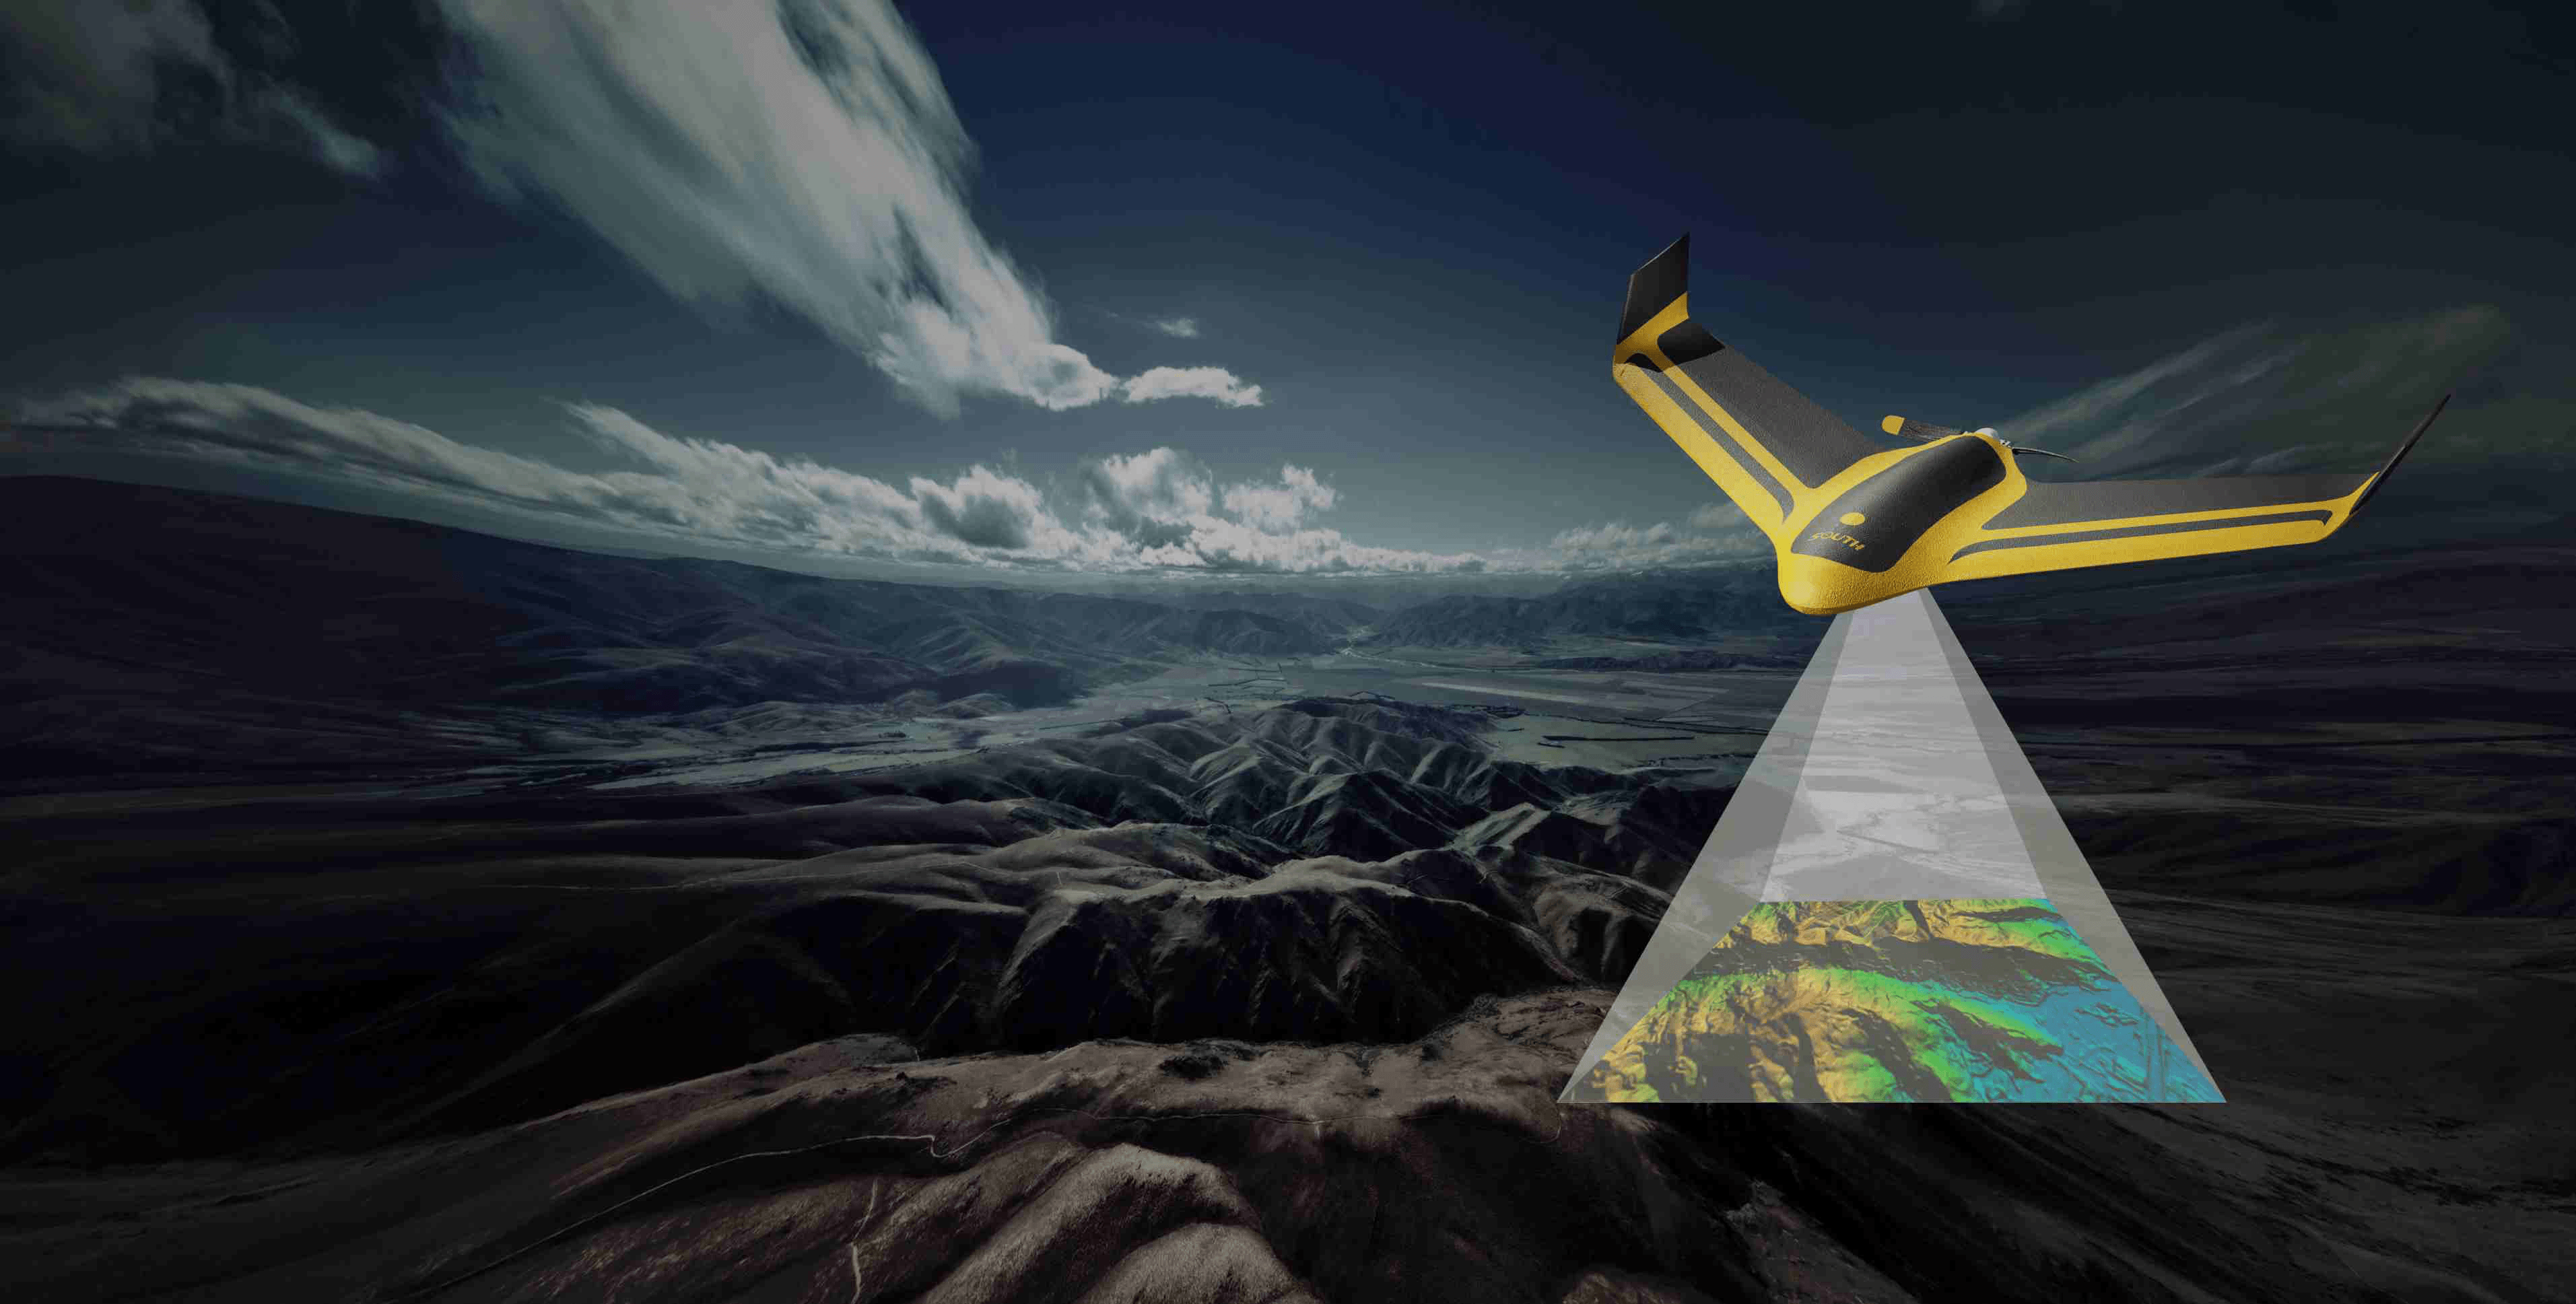
\includegraphics[width=0.3\textwidth]{han.png} 
		\label{subfig:png}
	} 
	\hspace{30pt}
	\subfloat[image2]
	{
		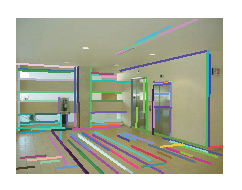
\includegraphics[width=0.2\textwidth]{HF.eps} 
		\label{subfig:eps}
	}
	\hspace{30pt}
	\subfloat[image3]
	{
		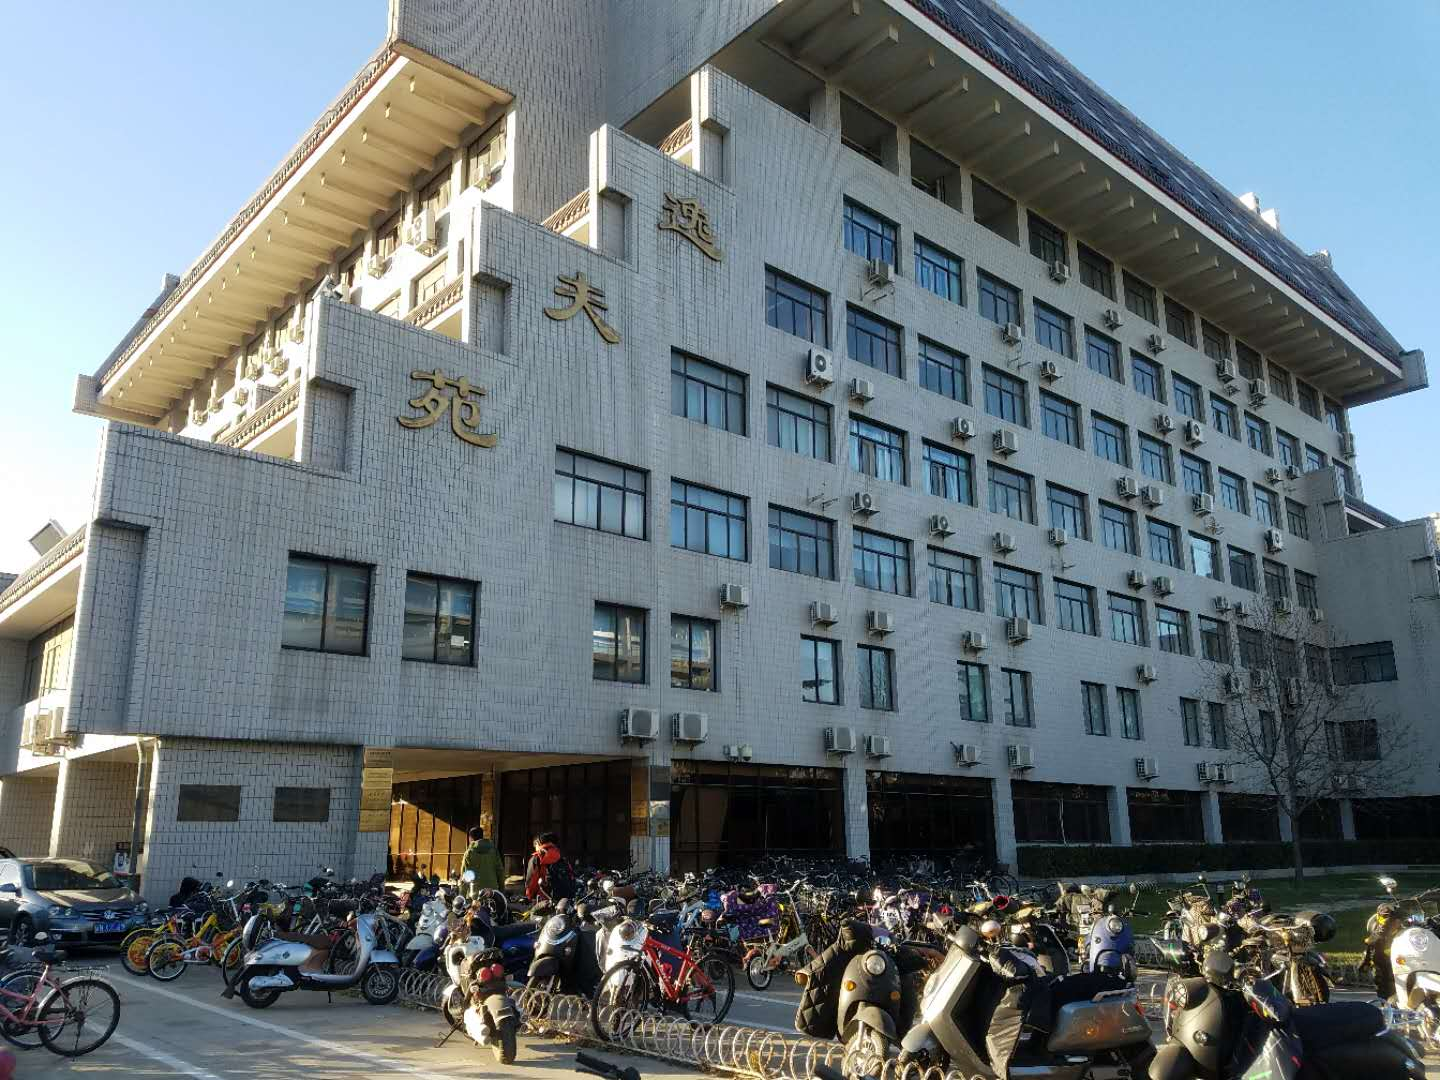
\includegraphics[width=0.2\textwidth]{build.jpg} 
		\label{subfig:jpg}
	}
	\caption{subfigures.}
	\label{fig:subfigures}
\end{figure}

\end{document}